\documentclass[12pt]{article}
\usepackage[utf8]{inputenc}
\usepackage{float}
\usepackage{amsmath}


\usepackage[hmargin=3cm,vmargin=6.0cm]{geometry}
%\topmargin=0cm
\topmargin=-2cm
\addtolength{\textheight}{6.5cm}
\addtolength{\textwidth}{2.0cm}
%\setlength{\leftmargin}{-5cm}
\setlength{\oddsidemargin}{0.0cm}
\setlength{\evensidemargin}{0.0cm}

%misc libraries goes here
\usepackage{tikz}
\usetikzlibrary{automata,positioning}

\begin{document}

\section*{Student Information } 
%Write your full name and id number between the colon and newline
%Put one empty space character after colon and before newline
Full Name : Yavuz Selim Yesilyurt \\
Id Number : 2259166 \\

% Write your answers below the section tags
\section*{Answer 1}

\subsection*{a.}
We can construct the bottom-up parser for $G$ as the following: \\

\begin{align*}
1-&((q_0,a,e),(q_0,a)) \\
2-&((q_0,b,e),(q_0,b)) \\
3-&((q_0,c,e),(q_0,S)) \\
4-&((q_0,e,e),(q_0,X)) \\
5-&((q_0,e,XbXSb),(q_0,S)) \\
6-&((q_0,e,XaXSa),(q_0,S)) \\
7-&((q_0,a,Xa),(q_0,X)) \\
8-&((q_0,a,Xb),(q_0,X)) \\
9-&((q_0,e,S),(q_1,e)) 
\end{align*} 
\subsection*{b.}
\begin{table}[H]
	\small
	\centering
	\begin{tabular}{|c|c|c|c|c|}	
	\hline
	$Step$ & $State$ & $Unread \ Input$ & $Stack$ & $Transition \ Used$\\
	\hline 
	1 & $q_0$ & $abbcbabbaa$ & $e$ & -\\			
	2 & $q_0$ & $bbcbabbaa$ & $a$ & 1\\	
	3 & $q_0$ & $bcbabbaa$  & $ba$ & 2\\
	4 & $q_0$ & $cbabbaa$   & $bba$ & 2\\
	5 & $q_0$ & $babbaa$   & $Sbba$ & 3\\	
	6 & $q_0$ & $babbaa$ & $XSbba$ & 4\\			
	7 & $q_0$ & $abbaa$ & $bXSbba$ & 2\\	
	8 & $q_0$ & $abbaa$  & $XbXSbba$ & 4\\
	9 & $q_0$ & $abbaa$   & $Sba$ & 5\\
	10 & $q_0$ & $bbaa$ & $aSba$ & 1\\			
	11 & $q_0$ & $bbaa$ & $XaSba$ & 4\\	
	12 & $q_0$ & $bbaa$  & $XSba$ & 7\\
	13 & $q_0$ & $baa$   & $bXSba$ & 2\\
	14 & $q_0$ & $baa$   & $XbXSba$ & 4\\	
	15 & $q_0$ & $baa$ & $Sa$ & 5\\			
	16 & $q_0$ & $aa$ & $bSa$ & 2\\	
	17 & $q_0$ & $aa$  & $abSa$ & 1\\
	18 & $q_0$ & $a$   & $XabSa$ & 4\\
	19 & $q_0$ & $a$ & $XbSa$ & 7\\			
	20 & $q_0$ & $a$ & $XSa$ & 8\\	
	21 & $q_0$ & $a$  & $aXSa$ & 1\\
	22 & $q_0$ & $e$   & $XaXSa$ & 4\\
	23 & $q_0$ & $e$   & $S$ & 6\\	
	24 & $q_1$ & $e$ & $e$ & 9\\			
	\hline 
	\end{tabular}
	\end{table}

\newpage
\section*{Answer 2}

\subsection*{a.}
We can define the Turing Machine which computes $f(x)$ as $M = (K,\Sigma,\delta_1, s, H)$, where
$K = \{s_0,odd,even,q_0,q_1,q_2,q_3,q_4,h\}$, $\Sigma = \{\sqcup,1,0,\triangleright\}$, $s = s_0$, $H = \{h\}
$ and the transition function is defined as follows;
\begin{align*}
&\delta_1(s_0,\sqcup) = (odd,\rightarrow) &&\delta_1(q_1,0) = (q_2,\rightarrow)\\
&\delta_1(odd,1) = (even,\rightarrow) &&\delta_1(q_2,1) = (q_2,0)\\
&\delta_1(odd,\sqcup) = (q_0,\leftarrow) &&\delta_1(q_2,0) = (q_3,\rightarrow) \\
&\delta_1(even,1) = (odd,\rightarrow) &&\delta_1(q_3,1) = (q_3,\rightarrow)\\
&\delta_1(even,\sqcup) = (h,1) &&\delta_1(q_3,\sqcup) = (q_0,\leftarrow) \\
&\delta_1(q_0,1) = (q_0,\sqcup) &&\delta_1(q_4,0) = (q_4,1) \\
&\delta_1(q_0,\sqcup) = (q_1,\leftarrow) &&\delta_1(q_4,1) = (q_4,\leftarrow)\\
&\delta_1(q_0,0) = (q_4,1) &&\delta_1(q_4,\sqcup) = (h,\sqcup)\\
&\delta_1(q_1,1) = (q_1,\leftarrow) \\
&\delta_1(q_1,\sqcup) = (q_2,\rightarrow)
\end{align*}
Note that the transition function also includes the functions of the form $\delta_1(y,\triangleright) 
= (s_1, \rightarrow)$ for every $y\in K_1-H_1$ trivially.
The machine defined above performs like this;\\\\
First, it goes right to find a 1. It keeps going right with reading 1 until it read a blank symbol. After reading blank symbol if machine is in the even state then it makes that blank symbol 1 and halts, but if the machine is in the odd state it goes one left to get the last 1, then it makes that 1 a blank symbol and keeps going left until it reads a blank symbol (actually it reaches to the blank symbol at the start), then it goes one right to access the first 1. After reaching the first 1 it replaces it with a 0 and again it goes to the last 1 to its right and again it replaces the last 1 with a blank symbol and comes to the first 1 again and replaces it with a 0. The machine keeps doing that until it sees blank symbol next to 0. After seeing this it just replaces all the 0's to its right to 1's and when it reaches to the blank symbol at first it halts.

\section*{Answer 3}
The set of languages decided by a semi-infinite tape, Move-restricted Turing Machines is equivalent to set of languages recognized by Finite Automatas, since the Move-restricted Turing Machines have neither the ability of moving its head left nor the ability of storing the information given by input string (stack behaviour). It can only read the input word from left to right and any modifications it would make onto input string would also be intraceable since it can not go back and inspect the value there and this is similar to behaviour of Finite Automatas, they also cant keep track of the memory of the word and cant read other parts of word. Therefore, it can be inferred that the class of languages decided by them is actually equivalent to class of languages recognized by Finite Automatas.

\section*{Answer 4}

\subsection*{a.}
We can define the Queue-based deterministic Turing Machine as $M = (K,\Sigma,\delta_1, s, H)$, where
$K = \{s_0,q_0,enqueue,dequeue,h\}$, $\Sigma = \{\sqcup,a,b,\triangleright\}$, $s = s_0$, $H = \{h\}
$ and the transition function is defined as follows (Note that this is just a general definition, for distinct languages, these definitions-K,$\Sigma$,s,H,$\delta$- may differ):
\begin{align*}
&\delta_1(s_0,input \ symbol) = (q_0,front \ symbol,rear \ symbol)\\
&\delta(q_0,X) = (dequeue,\sqcup,rear \ symbol) \\
&\delta(dequeue,input \ symbol) = (q_0,\rightarrow,rear \ symbol) \\
&\delta(q_0,a) = (enqueue,front \ symbol,\rightarrow) \\
&\delta(enqueue,a) = (q_0,front symbol,a) \\
&\delta(q_0,b) = (enqueue,front \ symbol,\rightarrow) \\
&\delta(enqueue,b) = (q_0,front symbol,b) \\
&\delta(q_0,\sqcup) = (h,front \ symbol,rear \ symbol)
\end{align*}

where $front \ symbol$ and $rear \ symbol$ $\in \Sigma$ and indicates what is under the front and rear heads at that moment respectively. \\

Note that we assume initially tape of the machine is filled with some string already stored inside and it has 2 heads front and rear, initially pointing to the start and the end of the word inside respectively. As the machine reads input instructions, it updates its content and heads accordingly. Machine has a main state $q_0$ and if the input instruction gives an X symbol, then machine will go to dequeue state and it will fulfill dequeue operation and return to the main state $q_0$. If the input instruction gives a symbol from $\Sigma - \{\sqcup,\triangleright\}$, the machine will go to enqueue state and it will fulfill enqueue operation with given symbol word and return to the main state $q_0$. And, if input instruction gives a $\sqcup$ symbol, the machine will halt. Also note that $Front$ and $Rear$ operations can be fulfilled through directly reading the symbol under $Front$ and $Rear$ heads at that moment.

\subsection*{b.}
Notion of configuration of Queue-based deterministic Turing Machine can be written as: \\
\begin{center}
$K \times \{\Sigma - \{\triangleright ,\sqcup \} \} \times \{\Sigma - \{\triangleright ,\sqcup \} \}^* \times \{\Sigma - \{\triangleright ,\sqcup \} \}$
\end{center}
Note that it refers to: (Current State, Symbol Under Front Head, Everything To The Right of the Front Head, Symbol Under Rear Head)
\subsection*{c.}
Yields-in-one-step relation of the machine can be written as: \\
\begin{center}
$(q_1,a_1,w_1,b_1) \vdash_M (q_2,a_2,w_2,b_2)$ \\
where $a_1,a_2,b_1,b_2\in \Sigma$ , and $\delta(q_1,input \ symbol) = (q_2,a_2,b_2)$
\end{center}

\subsection*{d.}
Church-Turing Thesis states that all computational devices-machines have the same power regarding computability. Any language, that is decided, semi-decided or any function that is computed by Queue-based deterministic Turing Machine can be decided, semi-decided or computed by a standard Turing Machine. To prove, we can mimick the transitions and operations that can be done in Queue-based TM, in standard TM as: \\

For front operation, we can give the first element of the string on the tape by going left until the reading head reads the start symbol or a blank symbol and then going one right, for rear operation, we can give the last element of the string on the tape by going right until the reading head reads a blank symbol and then going one left, For enqueue operation, we can operate rear operation first and go one more right and replace the blank symbol by the symbol that is needed to be enqueued, For dequeue operation, we can operate front operation first and replace the symbol under the reading head with a blank symbol and going one right. 

\subsection*{e.}
We can define the Queue-based deterministic Turing Machine for $L = \{wcw : w \in \{a,b\}^*\}$ as $M = (K,\Sigma,\delta, s, H)$, where
$K = \{s_0,enqueue,dequeue,h\}$, $\Sigma = \{\sqcup,a,b,c,\triangleright\}$, $s = s_0$, $H = \{h\}
$ and the transition function is defined as follows;
\begin{align*}
&\delta(s_0,a,\triangleright,\triangleright) = (enqueue,a,\rightarrow,\rightarrow)\\
&\delta(s_0,b,\triangleright,\triangleright) = (enqueue,b,\rightarrow,\rightarrow)\\
&\delta(enqueue,a,\sqcup,\sqcup) = (enqueue,\rightarrow,a,\rightarrow)\\
&\delta(enqueue,b,\sqcup,\sqcup) = (enqueue,\rightarrow,b,\rightarrow)\\
&\delta(enqueue,a,front \ symbol,rear \ symbol) = (enqueue,\rightarrow,front \ symbol,\rightarrow)\\
&\delta(enqueue,b,front \ symbol,rear \ symbol) = (enqueue,\rightarrow,front \ symbol,\rightarrow)\\
&\delta(enqueue,a,front \ symbol,\sqcup) = (enqueue,\rightarrow,front \ symbol,a)\\
&\delta(enqueue,b,front \ symbol,\sqcup) = (enqueue,\rightarrow,front \ symbol,b)\\
&\delta(enqueue,c,front \ symbol,rear \ symbol) = (dequeue,\rightarrow,front \ symbol,rear \ symbol)\\
&\delta(dequeue,a,a,rear \ symbol) = (dequeue,\rightarrow,\sqcup,rear \ symbol)\\
&\delta(dequeue,b,b,rear \ symbol) = (dequeue,\rightarrow,\sqcup,rear \ symbol)\\
&\delta(dequeue,a,\sqcup,rear \ symbol) = (dequeue,\rightarrow,\rightarrow,rear \ symbol)\\
&\delta(dequeue,b,\sqcup,rear \ symbol) = (dequeue,\rightarrow,\rightarrow,rear \ symbol)\\
&\delta(dequeue,\sqcup,\sqcup,\sqcup) = (h,\sqcup,\sqcup,\sqcup) \\
\end{align*}

where $front \ symbol$ and $rear \ symbol$ $\in \Sigma$ and indicates what is under the front and rear heads at that moment respectively. \\

Note that initially front and rear heads are pointing to the start symbol. Firstly, as the Machine reads input words, it enqueues each of them until it reads a c symbol and updates its heads and content accordingly. After reading a c, it will go to dequeue state and as it reads the other half of the input, it will check if the symbol under the front head and input matches and if they match it will dequeue the and update its front head accordingly. When machine reads a blank symbol it will check if the symbol under its front and rear head is a blank symbol (i.e. the heads point the same symbol and tape is empty) and if it is, then the machine will halt.

\section*{Answer 5}

\subsection*{a.}

\begin{center}
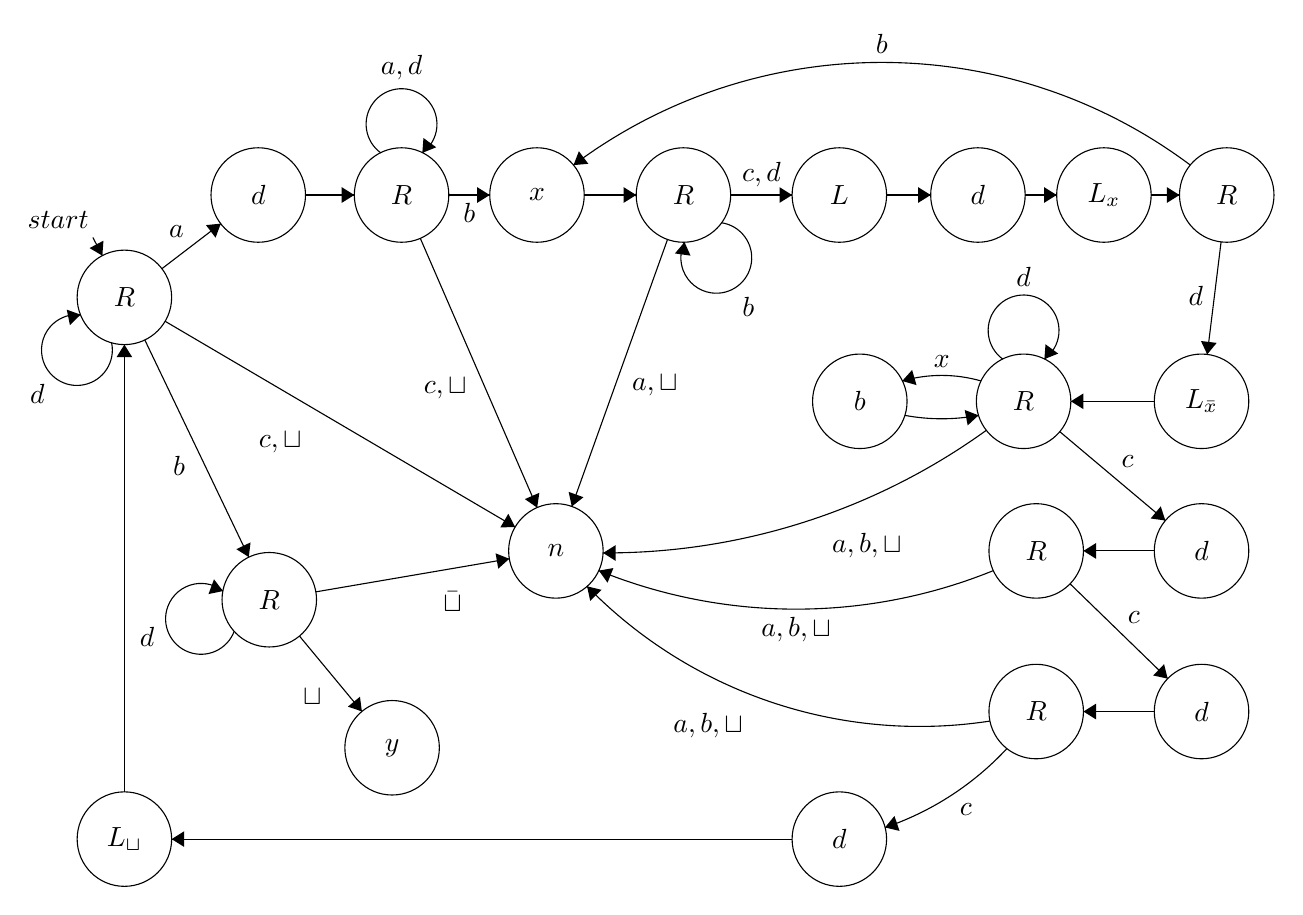
\begin{tikzpicture}[scale=0.2]
\tikzstyle{every node}+=[inner sep=0pt]
\draw [black] (6.3,-20) circle (3);
\draw (6.3,-20) node {$R$};
\draw [black] (14.8,-13.5) circle (3);
\draw (14.8,-13.5) node {$d$};
\draw [black] (23.9,-13.5) circle (3);
\draw (23.9,-13.5) node {$R$};
\draw [black] (32.5,-13.5) circle (3);
\draw (32.5,-13.5) node {$x$};
\draw [black] (41.8,-13.5) circle (3);
\draw (41.8,-13.5) node {$R$};
\draw [black] (51.7,-13.5) circle (3);
\draw (51.7,-13.5) node {$L$};
\draw [black] (60.5,-13.5) circle (3);
\draw (60.5,-13.5) node {$d$};
\draw [black] (68.5,-13.5) circle (3);
\draw (68.5,-13.5) node {$L_x$};
\draw [black] (76.3,-13.5) circle (3);
\draw (76.3,-13.5) node {$R$};
\draw [black] (33.7,-36.1) circle (3);
\draw (33.7,-36.1) node {$n$};
\draw [black] (74.7,-26.6) circle (3);
\draw (74.7,-26.6) node {$L_{\bar{x}}$};
\draw [black] (63.4,-26.6) circle (3);
\draw (63.4,-26.6) node {$R$};
\draw [black] (53,-26.6) circle (3);
\draw (53,-26.6) node {$b$};
\draw [black] (74.7,-36.1) circle (3);
\draw (74.7,-36.1) node {$d$};
\draw [black] (64.2,-36.1) circle (3);
\draw (64.2,-36.1) node {$R$};
\draw [black] (74.7,-46.3) circle (3);
\draw (74.7,-46.3) node {$d$};
\draw [black] (64.2,-46.3) circle (3);
\draw (64.2,-46.3) node {$R$};
\draw [black] (51.7,-54.4) circle (3);
\draw (51.7,-54.4) node {$d$};
\draw [black] (6.3,-54.4) circle (3);
\draw (6.3,-54.4) node {$L_{\sqcup}$};
\draw [black] (15.5,-39.2) circle (3);
\draw (15.5,-39.2) node {$R$};
\draw [black] (23.3,-48.6) circle (3);
\draw (23.3,-48.6) node {$y$};
\draw [black] (4.3,-16.2) -- (4.9,-17.35);
\draw (2.09,-15.69) node [above] {$start$};
\fill [black] (4.9,-17.35) -- (4.97,-16.4) -- (4.09,-16.87);
\draw [black] (8.68,-18.18) -- (12.42,-15.32);
\fill [black] (12.42,-15.32) -- (11.48,-15.41) -- (12.09,-16.21);
\draw (9.6,-16.25) node [above] {$a$};
\draw [black] (17.8,-13.5) -- (20.9,-13.5);
\fill [black] (20.9,-13.5) -- (20.1,-13) -- (20.1,-14);
\draw [black] (22.577,-10.82) arc (234:-54:2.25);
\draw (23.9,-6.25) node [above] {$a,d$};
\fill [black] (25.22,-10.82) -- (26.1,-10.47) -- (25.29,-9.88);
\draw [black] (26.9,-13.5) -- (29.5,-13.5);
\fill [black] (29.5,-13.5) -- (28.7,-13) -- (28.7,-14);
\draw (28.2,-14) node [below] {$b$};
\draw [black] (35.5,-13.5) -- (38.8,-13.5);
\fill [black] (38.8,-13.5) -- (38,-13) -- (38,-14);
\draw [black] (44.214,-15.261) arc (81.6215:-206.3785:2.25);
\draw (45.92,-19.98) node [below] {$b$};
\fill [black] (41.87,-16.49) -- (41.26,-17.21) -- (42.25,-17.35);
\draw [black] (40.79,-16.32) -- (34.71,-33.28);
\fill [black] (34.71,-33.28) -- (35.45,-32.69) -- (34.51,-32.35);
\draw (38.51,-25.57) node [right] {$a,\sqcup$};
\draw [black] (25.09,-16.25) -- (32.51,-33.35);
\fill [black] (32.51,-33.35) -- (32.65,-32.41) -- (31.73,-32.81);
\draw (28.07,-25.77) node [left] {$c,\sqcup$};
\draw [black] (44.8,-13.5) -- (48.7,-13.5);
\fill [black] (48.7,-13.5) -- (47.9,-13) -- (47.9,-14);
\draw (46.75,-13) node [above] {$c,d$};
\draw [black] (54.7,-13.5) -- (57.5,-13.5);
\fill [black] (57.5,-13.5) -- (56.7,-13) -- (56.7,-14);
\draw [black] (63.5,-13.5) -- (65.5,-13.5);
\fill [black] (65.5,-13.5) -- (64.7,-13) -- (64.7,-14);
\draw [black] (71.5,-13.5) -- (73.3,-13.5);
\fill [black] (73.3,-13.5) -- (72.5,-13) -- (72.5,-14);
\draw [black] (34.816,-11.595) arc (126.80351:53.19649:32.69);
\fill [black] (34.82,-11.6) -- (35.76,-11.52) -- (35.16,-10.72);
\draw (54.4,-4.58) node [above] {$b$};
\draw [black] (75.94,-16.48) -- (75.06,-23.62);
\fill [black] (75.06,-23.62) -- (75.66,-22.89) -- (74.66,-22.77);
\draw (74.83,-19.92) node [left] {$d$};
\draw [black] (71.7,-26.6) -- (66.4,-26.6);
\fill [black] (66.4,-26.6) -- (67.2,-27.1) -- (67.2,-26.1);
\draw [black] (55.693,-25.31) arc (106.09686:73.90314:9.042);
\fill [black] (55.69,-25.31) -- (56.6,-25.57) -- (56.32,-24.61);
\draw (58.2,-24.46) node [above] {$x$};
\draw [black] (60.543,-27.492) arc (-79.39967:-100.60033:12.737);
\fill [black] (60.54,-27.49) -- (59.66,-27.15) -- (59.85,-28.13);
\draw [black] (61.033,-28.442) arc (-54.19775:-90.3269:41.199);
\fill [black] (36.7,-36.23) -- (37.49,-36.73) -- (37.5,-35.73);
\draw (53.45,-34.96) node [below] {$a,b,\sqcup$};
\draw [black] (62.077,-23.92) arc (234:-54:2.25);
\draw (63.4,-19.35) node [above] {$d$};
\fill [black] (64.72,-23.92) -- (65.6,-23.57) -- (64.79,-22.98);
\draw [black] (65.7,-28.53) -- (72.4,-34.17);
\fill [black] (72.4,-34.17) -- (72.11,-33.27) -- (71.47,-34.04);
\draw (70,-30.86) node [above] {$c$};
\draw [black] (71.7,-36.1) -- (67.2,-36.1);
\fill [black] (67.2,-36.1) -- (68,-36.6) -- (68,-35.6);
\draw [black] (61.475,-37.352) arc (-67.90323:-112.09677:33.296);
\fill [black] (36.43,-37.35) -- (36.98,-38.12) -- (37.35,-37.19);
\draw (48.95,-40.3) node [below] {$a,b,\sqcup$};
\draw [black] (66.35,-38.19) -- (72.55,-44.21);
\fill [black] (72.55,-44.21) -- (72.32,-43.29) -- (71.63,-44.01);
\draw (70.41,-40.72) node [above] {$c$};
\draw [black] (71.7,-46.3) -- (67.2,-46.3);
\fill [black] (67.2,-46.3) -- (68,-46.8) -- (68,-45.8);
\draw [black] (61.263,-46.905) arc (-81.27787:-135.7047:29.491);
\fill [black] (35.68,-38.35) -- (35.88,-39.27) -- (36.6,-38.57);
\draw (43.37,-46.39) node [below] {$a,b,\sqcup$};
\draw [black] (62.341,-48.65) arc (-42.90766:-71.20587:18.855);
\fill [black] (54.6,-53.66) -- (55.52,-53.88) -- (55.2,-52.93);
\draw (59.73,-52.14) node [below] {$c$};
\draw [black] (48.7,-54.4) -- (9.3,-54.4);
\fill [black] (9.3,-54.4) -- (10.1,-54.9) -- (10.1,-53.9);
\draw [black] (6.3,-51.4) -- (6.3,-23);
\fill [black] (6.3,-23) -- (5.8,-23.8) -- (6.8,-23.8);
\draw [black] (5.487,-22.876) arc (11.95432:-276.04568:2.25);
\draw (0.77,-25.5) node [below] {$d$};
\fill [black] (3.52,-21.1) -- (2.64,-20.78) -- (2.84,-21.76);
\draw [black] (8.89,-21.52) -- (31.11,-34.58);
\fill [black] (31.11,-34.58) -- (30.68,-33.74) -- (30.17,-34.61);
\draw (16.2,-28.55) node [below] {$c,\sqcup$};
\draw [black] (7.6,-22.71) -- (14.2,-36.49);
\fill [black] (14.2,-36.49) -- (14.31,-35.56) -- (13.41,-35.99);
\draw (10.19,-30.67) node [left] {$b$};
\draw [black] (13.276,-41.196) arc (-20.35775:-308.35775:2.25);
\draw (8.23,-41.57) node [left] {$d$};
\fill [black] (12.56,-38.65) -- (11.99,-37.9) -- (11.64,-38.84);
\draw [black] (18.46,-38.7) -- (30.74,-36.6);
\fill [black] (30.74,-36.6) -- (29.87,-36.25) -- (30.04,-37.23);
\draw (27.14,-38.68) node [below] {$\bar{\sqcup}$};
\draw [black] (17.42,-41.51) -- (21.38,-46.29);
\fill [black] (21.38,-46.29) -- (21.26,-45.36) -- (20.49,-45.99);
\draw (18.85,-45.34) node [left] {$\sqcup$};
\end{tikzpicture}
\end{center}

\subsection*{b.}
Let $G = (V,\Sigma,R,S)$ be the grammar and $V = (a,b,c,S,X,R)$, $\Sigma = (a,b,c)$, $R \subseteq (V - \Sigma) \times V^*$, The rules are:

\begin{align*}
S &\rightarrow b | abbcccX \\
X &\rightarrow RX | e \\
cR &\rightarrow Rcccc \\
cR &\rightarrow Rc \\
bR &\rightarrow Rbb \\ 
aR &\rightarrow Raa \\
aR &\rightarrow Ra \\ 
R &\rightarrow e \\
\end{align*}

\section*{Answer 6}

\subsection*{a.}
With the information given to us, let's find out more about these 5 languages: \\

Since a \textbf{regular grammar} can generate all strings in $L_1$ we can deduce that $L_1$ is a regular language. Since a Finite Automata can recognize $L_1$, a proper $M_1$ can be written for $L_1$. \\

If a \textbf{deterministic top-down parser} can be built for CFG whose language is $L_2$ then we can say that $L_2$ is a deterministic context-free language. Since a Deterministic Push Down Automata can recognize $L_2$, a proper $M_2$ can be written for $L_2$.\\

$L_3$ is a context-free language since a (inherently ambiguous) context-free grammar can be provided for this language. Since a Push Down Automata can recognize $L_3$, a proper $M_3$ can be written for $L_3$.\\

Since a TM M decides the resulting language ($\bar{L_4}\cap \bar{L(a^*b^*)}$) we can say it is recursive. Since $\bar{L(a^*b^*)}$ is a regular language, for result to be recursive, left-handside ($\bar{L_4}$) must be recursive. Since recursive languages are closed under complementation, we can deduce that $L_4$ is a recursive language. Since it is recursive, it can be decided by some TM $M_4$.\\

We know that the class of languages generated by unrestricted grammars is equivalent to class of languages that is semi-decided by Turing Machines. Given an unrestricted grammar, a Turing machine is simple enough to construct, as a two-tape nondeterministic Turing machine. Since $L_5$ is also generated by an unrestricted grammar, we can deduce that it is a recursively enumerable language. Since it is recursively enumerable, it can be semi-decided by some TM $M_5$.\\

Therefore, yes, all 5 TM's for languages exists.

\subsection*{b.}
Church-Turing Thesis states that an algorithm corresponds to a TM that halts on every input. Also we know that, everything that can be computed has an algorithm. In part a we showed that, for these 5 languages corresponding TM's exists and they are all in the class of languages that is eventually decidable/semi-decidable. Therefore all of them can be generated by a (unrestricted) grammar, we can make the computation, so we  deduce that there always exists algorithms for these languages, they are computable.
\subsection*{c.}
Let's first decide whether $L$ is undecidable or not: \\

We know that $L_1$ is regular and $L_2$ is DCFL. Since DCFLs are closed under complementation $\bar{L_2}$ is also a DCFL. Since DCFLs are also closed under concatenation, $\bar{L_2}L_1$ is also a DCFL. We know that $L_5$ is recursively enumerable, since recursively enumerable languages are closed under intersection and Kleene Star $(\bar{L_2}L_1 \cap L_5)^*$ is also a recursively enumerable language. We know that $L_3$ is CFL and $L_4$ is recursive. Since CFLs are closed under Kleene Star $L_3^*$ is also a CFL and since recursive languages are closed under complementation $\bar{L_4}$ is also a recursive language. Since recursive languages are closed under concatenation $L_3^*\bar{L_4}$ is also recursive. Finally, since recursively enumerable languages are closed under union, $L = (\bar{L_2}L_1 \cap L_5)^* \cup L_3^*\bar{L_4}$ is also a recursively enumerable language. So $L$ is semi-decidable by some TM $M$. $M$ will accept a string, for given inputs, it also may not halt.
\subsection*{d.}
We can't. Because complement of recursively enumerable languages are not necessarily recursively enumerable, they may be undecidable. Let us justify that by reaching a contradiction for assuming that an undecidable language is a recursively enumerable language: \\

Let $H = \{"M""w"|\textit{TM M halts on input w}\}$, $H$ is semi-decided by Universal Turing Machine, therefore it is recursively enumerable. Suppose it is recursive, then there exists a TM $M_0$ that decides $H$, consider $H_1 = \{"M"|\textit{TM M halts on "M"}\}$, if $H$ is recursive, then $H_1$ is also recursive, if $H_1$ is recursive, then so does its complement, $\bar{H_1}=\{w|\textit{w is not encoding of a TM or}$ $\textit{does not halt on itself}\}$. There must be some TM $M^*$ that semi-decides $\bar{H_1}$ (if it is recursive, it also must be recursively enumerable). But at this point we reach a contradiction since, $"M^*"\in \bar{H_1}$ iff $M^*$ does halt on $"M^*"$ and also by definition of $\bar{H_1}$, $"M^*"\in \bar{H_1}$ iff $M^*$ does not halt on $"M^*"$. So we prove that $\bar{H_1}$ is not recursively enumerable, $H_1$ is not recursive and $H$ is not recursive, yet the only conclusion that we are interested is that $\bar{H_1}$ is not recursively enumerable and we can't come up with a TM for $\bar{H_1}$, which also proves the statement that "We always come up with a TM that semi-decides $\bar{L}$" is not true.

%Do not submit solutions for Question 7, yet do solve it.


\end{document}

​

